\documentclass[tikz,border=10pt]{standalone}
\usepackage{amsmath}
\usetikzlibrary{arrows.meta, positioning, calc, decorations.pathreplacing}
\definecolor{c1}{HTML}{000000}
\definecolor{c2}{HTML}{233D4D}
\definecolor{c3}{HTML}{FE7F2D}
\definecolor{c4}{HTML}{EAECF0}
\definecolor{axiscolor}{HTML}{333333}
\definecolor{labelcolor}{HTML}{5F6B75}
\begin{document}
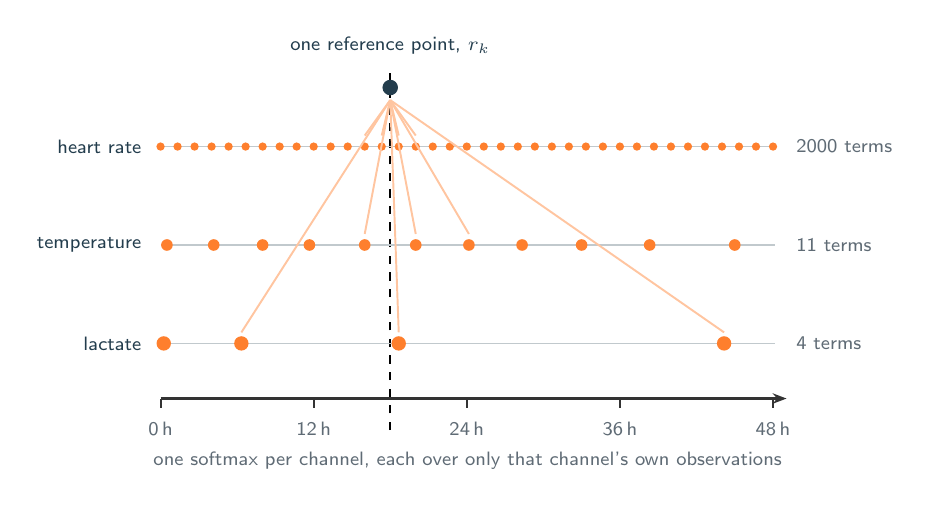
\begin{tikzpicture}[
    every node/.style={font=\sffamily},
    lab/.style={font=\sffamily\scriptsize, text=labelcolor},
    tag/.style={font=\sffamily\scriptsize, text=c2},
    hot/.style={font=\sffamily\scriptsize, text=c3!85!black},
]
\def\X#1{2.30 + #1*0.002700}

% the one reference point
\draw[c1, line width=0.9pt, dashed] ({\X{1080}}, 0.95) -- ({\X{1080}}, 5.55);
\node[tag, anchor=south] at ({\X{1080}}, 5.60) {one reference point, $r_k$};
\fill[c2] ({\X{1080}}, 5.30) circle (2.8pt);

% three channels, each with its own observations
\foreach \y/\name/\n in {4.55/heart rate/{2000 terms},
                         3.30/temperature/{11 terms},
                         2.05/lactate/{4 terms}}{
    \node[tag, anchor=east] at (2.18, \y) {\name};
    \draw[c2!28, line width=0.6pt] (2.30, \y) -- (10.10, \y);
    \node[lab, anchor=west] at (10.25, \y) {\n};
}
\foreach \m in {0,80,...,2880}{
    \fill[c3] ({\X{\m}}, 4.55) circle (1.5pt);
}
\foreach \m in {30, 250, 480, 700, 960, 1200, 1450, 1700, 1980, 2300, 2700}{
    \fill[c3] ({\X{\m}}, 3.30) circle (2.1pt);
}
\foreach \m in {15, 380, 1120, 2650}{
    \fill[c3] ({\X{\m}}, 2.05) circle (2.6pt);
}

% each channel gets its own fan from the same reference point
\foreach \y/\ms in {4.55/{960,1040,1120,1200}, 3.30/{960,1200,1450}, 2.05/{380,1120,2650}}{
    \foreach \m in \ms {
        \draw[c3!45, line width=0.7pt] ({\X{1080}}, 5.14) -- ({\X{\m}}, {\y+0.14});
    }
}

\node[lab, anchor=north, align=center] at (6.20, 0.80)
    {one softmax per channel, each over only that channel's own observations};

\draw[axiscolor, line width=0.8pt, -{Stealth[length=5pt]}] (2.30, 1.35) -- (10.25, 1.35);
\foreach \h in {0, 12, 24, 36, 48}{
    \pgfmathsetmacro\m{\h*60}
    \draw[axiscolor, line width=0.7pt] ({\X{\m}}, 1.35) -- ({\X{\m}}, 1.23);
    \node[lab, anchor=north] at ({\X{\m}}, 1.17) {\h\,h};
}
\end{tikzpicture}
\end{document}
